\documentclass[a4paper,10pt]{article}
\usepackage[utf8]{inputenc}
\usepackage{graphicx}
%opening
\title{}
\author{}

\begin{document}


\section{Encontros}

* Preferem horários fixos. 
* Enquete no moodle sobre horários.

\section{Questões}
\begin{eqnarray*}
 \vec{u} &=& u_1\vec{i} + u_2\vec{j} + u_3\vec{k}\\
 \vec{v} &=& v_1\vec{i} + v_2\vec{j} + v_3\vec{k}
\end{eqnarray*}

Como $\vec{u}$ e $\vec{v}$ estão no plano XY, $u_3=v_3=0$. 

Como $\|\vec{v}\|=0$, $\vec{v}=\vec{0}$.

Já $\vec{u}$ é unitario, então $u_1^2+u_2^2=1$.
$$u_1=\cos(\theta),~~u_2=\sin(\theta).$$

Obs.: Quando $\theta=0$, $\vec{u}=\vec{i}$.
Quando $\theta=\pi/2$, $\vec{u}=\vec{j}$,

\section{Produto misto}
\begin{eqnarray*}
 \vec{u}\times  \vec{v} \cdot \vec{w}=(\vec{u}\times  \vec{v}) \cdot \vec{w}=\underbrace{\vec{u}\times(  \vec{v} \cdot \vec{w})}_{ERRADO}
\end{eqnarray*}


\begin{eqnarray*}
\vec{u}&=&\vec{i}+2\vec{j}+3\vec{k}\\
\vec{v}&=&\vec{i}       -\vec{k}\\
\vec{w}&=&\vec{i}+2\vec{j}+\vec{k}\\
\end{eqnarray*}

\begin{eqnarray*}
\left|\begin{array}{ccc}
1&2&3\\       
1&0&-1\\
1&2&1
      \end{array}
\right| = 1\cdot 0 \cdot 1 + 2\cdot(-1)\cdot1 + 3\cdot 1\cdot 2 - 3\cdot 0\cdot 1 - 2\cdot 1\cdot 1 - 1 \cdot (-1) \cdot 2
\end{eqnarray*}

\section{Ângulo entre vetores}

Usaremos:
$$\vec{u}\cdot\vec{v} = \|u\|\|v\|\cos(\alpha)$$
$$|\vec{u}\times\vec{v}| = \|u\|\|v\|\sin(\alpha)$$


\section{Funções vetoriais}

$$\vec{u}(t) = u_1(t)\vec{i}+u_2(t)\vec{j}+u_3(t)\vec{k}$$

Exemplo: vetor posição.
$$\vec{r}(t) = x(t)\vec{i}+y(t)\vec{j}+z(t)\vec{k}$$

A velocidade é a derivada:
$$\vec{v}(t) = x'(t)\vec{i}+y'(t)\vec{j}+z'(t)\vec{k}$$

Teorema:
Se $\|\vec{r}(t)\|$ é constante, então:
$$\vec{r}(t)\cdot \vec{r}\!~'(t)=0$$


Aplicação na cinemática:
Se a velocidade de uma partícula tem módulo constante, isto é, velocidade escalar constante, então:
$$\vec{v}(t)\cdot \vec{v}\!~'(t)=\vec{v}(t)\cdot \vec{a}(t)=0$$

Generalização:
Se $\vec{v}(t)=v(t)\vec{T}(t)$
onde $\vec{T}(t)$ é o vetor tangente unitário dado por:
$$\vec{T}(t) = \frac{\vec{r}~\!'(t)}{\|\vec{r}~\!'(t)\|} $$

Diferenciando, temos:
\begin{eqnarray*}
 \vec{a}&=&\vec{v}~\!'(t)=\frac{d}{dt}\left[v(t)\vec{T}(t)\right]\\
 &=&\underbrace{v'(t)\vec{T}(t)}_{tangencial}+\underbrace{v(t)\vec{T}'(t)}_{normal}
\end{eqnarray*}
Observação. Como $\|\vec{T}(t)\|=1$, o teorema citado anteriormente garante que $\vec{T}(t)\cdot\vec{T}'(t)=0$.

\section{Curvatura}
A curvatura de uma curva descrita por $\vec{r}(t)$ é dada por:
$$\kappa(t) = \left\|\frac{d}{ds}\vec{T}(s)\right\|$$
onde $s(t)$ é o comprimento da curva.

\subsection{Circunferência}

\begin{eqnarray*}
\vec{r}(t)&=&\cos(t)\vec{i}+\sin(t)\vec{j} \\
\vec{r}~\!'(t)&=&-\sin(t)\vec{i}+\cos(t)\vec{j} \\
\|\vec{r}~\!'(t)\|&=&\sqrt{\sin^2(t)+\cos^2(t)}=1 \\
\end{eqnarray*}
Assim:
$$\vec{T}(t) = \frac{\vec{r}~\!'(t)}{\|\vec{r}~\!'(t)\|}=-\sin(t)\vec{i}+\cos(t)\vec{j}.$$
\begin{eqnarray*}
\kappa(t) &=& \left\|\frac{d}{ds}\vec{T}(s)\right\|\\
&=&\left\|\frac{d}{dt}\vec{T}(t)\right\|/ \frac{ds}{dt}\\
&=&\left\|\frac{d}{dt}\vec{T}(t)\right\|/ \|\vec{r}~\!'(t)\|\\
&=&\left\|\frac{d}{dt}\vec{T}(t)\right\|\\
&=&\left\|-\cos(t)\vec{i}-\sin(t)\vec{j}\right\|=1\\
\end{eqnarray*}



\section{Vetores $\vec{T}$-$\vec{N}$-$\vec{B}$ (24/agosto)}
\begin{center}
 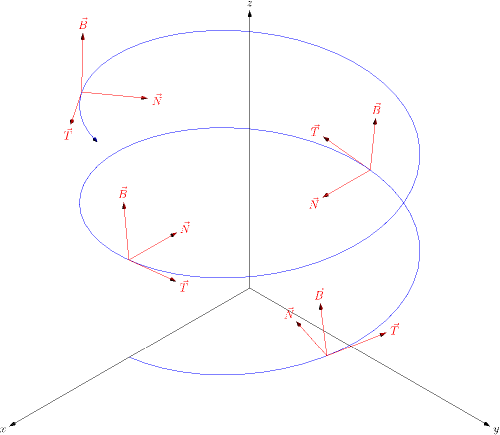
\includegraphics[width=7cm]{figs/helice_TNB.png}
 \end{center}

 \subsection{Vetor tangente unitário}
 Se uma curva é parametrizada pela função $\vec{r}(t)=x(t)\vec{i}+y(t)\vec{j}+z(t)\vec{k}$.
 
 Definimos o vetor tangente unitário:
 $$\vec{T}(t) = \frac{\vec{r}~\!'(t)}{\|\vec{r}~\!'(t)\|},~~\vec{r}~\!'(t)\neq \vec{0}.$$

 
 \subsection{Vetor normal unitário}
 Definimos o vetor normal unitário como:
 $$\vec{N}(t) = \frac{\vec{T}~\!'(t)}{\|\vec{T}~\!'(t)\|},~~\vec{T}~\!'(t)\neq \vec{0}.$$

  Obs: $\vec{N}(t)\cdot \vec{T}(t)=0$ porque $\vec{T}(t)$ tem norma constante. 
 

 
\subsubsection{Aplicação na cinemática}
Se a velocidade de uma partícula é a função $\vec{v}(t)$, então podemos escrever:
 $$\vec{v}(t)=v(t)\vec{T}(t)$$
onde $\vec{T}(t)$ é o vetor tangente unitário dado por:
$$\vec{T}(t) = \frac{\vec{r}~\!'(t)}{\|\vec{r}~\!'(t)\|}=\frac{\vec{v}(t)}{\|\vec{v}(t)\|} $$

Diferenciando, temos:
\begin{eqnarray*}
 \vec{a}&=&\vec{v}~\!'(t)=\frac{d}{dt}\left[v(t)\vec{T}(t)\right]\\
 &=&\underbrace{v'(t)\vec{T}(t)}_{tangencial}+\underbrace{v(t)\vec{T}'(t)}_{normal}
\end{eqnarray*}
Como $\vec{N}(t) = \frac{\vec{T}~\!'(t)}{\|\vec{T}~\!'(t)\|}$, obtemos:
\begin{eqnarray*}
 \vec{a}&=&\underbrace{v'(t)\vec{T}(t)}_{tangencial}+\underbrace{v(t)\|\vec{T}~\!'(t)\|\vec{N}(t)}_{normal}
\end{eqnarray*}
 
\subsection{Vetor binormal unitário}
O vetor binormal unitário é definido como:

 $$\vec{B}(t)=\vec{T}(t)\times\vec{N}(t)$$

 Obs: $\vec{T}(t)\times\vec{N}(t)\cdot \vec{T}(t) = \vec{T}(t)\times\vec{N}(t)\cdot \vec{N}(t)=0$ e
 $$\|\vec{T}(t)\times\vec{N}(t)\|=\|\vec{T}(t)\|\|\vec{N}(t)\|\sin(\alpha)=1\cdot 1 \cdot 1=1$$
 %\subsection{Hélice circular uniforme}

\subsection{Hélice}
Seja  hélice circular uniforme dada por:
$$\vec{r}(t)=\cos(t)\vec{i}+\sin(t)\vec{j}+ t\vec{k}$$
isto é:
\begin{eqnarray*}
 x(t)&=&\cos(t)\\
 y(t)&=&\sin(t)\\
 z(t)&=&t
\end{eqnarray*}

$$\vec{r}\!~'(t)=-\sin(t)\vec{i}+\cos(t)\vec{j}+ \vec{k}$$

A norma é dada por:
$$\|\vec{r}\!~'(t)\|=\sqrt{\sin^2(t)+\cos^2(t)+1}=\sqrt{2}$$

Assim:
$$\vec{T}(t)=\frac{-\sin(t)\vec{i}+\cos(t)\vec{j}+ \vec{k}}{\sqrt{2}}$$

Para calcular $\vec{N}$, derivamos $\vec{T}$:

$$\vec{T}~\!'(t)=\frac{-\cos(t)\vec{i}-\sin(t)\vec{j}}{\sqrt{2}}$$
e
$$\|\vec{T}~\!'(t)\|=\frac{\sqrt{\cos^2(t)+\sin^2(t)}}{\sqrt{2}}=\frac{1}{\sqrt{2}}$$
assim:
$$\vec{N}(t) = \frac{\vec{T}~\!'(t)}{\|\vec{T}~\!'(t)\|}=-\cos(t)\vec{i}-\sin(t)\vec{j}$$


Finalmente o vetor binormal unitário é dado por:
$$\vec{B}(t)= \vec{T}(t)\times \vec{N}(t)$$

\begin{eqnarray*}
 \vec{B}(t)&=&\frac{1}{\sqrt{2}}\left|
 \begin{array}{ccc}
\vec{i}&  \vec{j}&\vec{k}\\
-\sin(t)&\cos(t)&1\\
-\cos(t)&-\sin(t)&0
 \end{array}
 \right|\\
 &=&\frac{1}{\sqrt{2}}\left[\vec{i}\left(0+\sin(t)\right)+\vec{j}\left(-\cos(t)+0\right)+\vec{k}\left(\sin^2(t)+\cos^2(t)\right)\right]\\
 &=&\frac{1}{\sqrt{2}}\left[\sin(t)\vec{i}-\cos(t)\vec{j}+\vec{k}\right]
\end{eqnarray*}



\begin{center}
 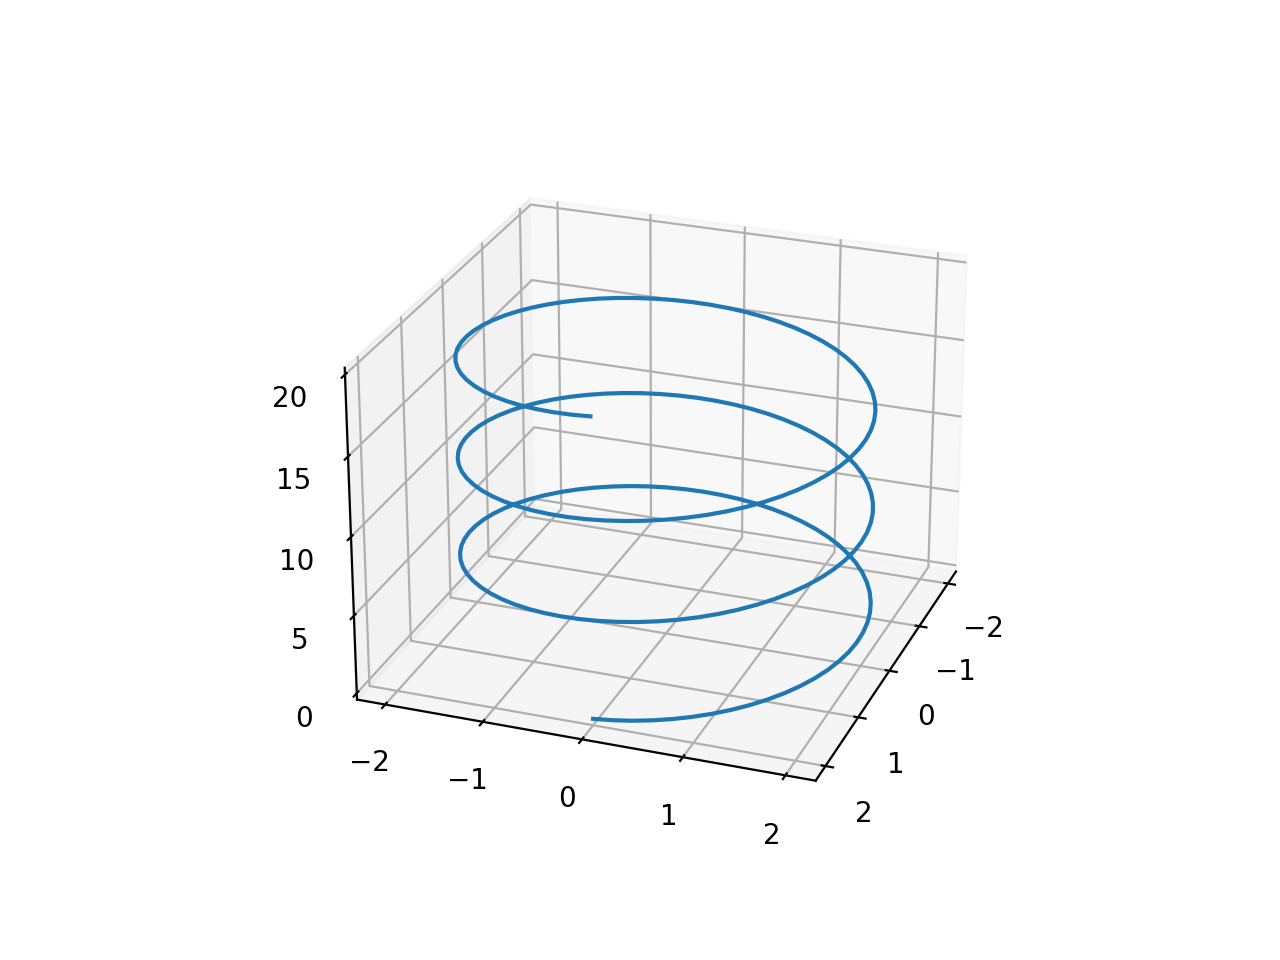
\includegraphics[width=10cm]{figs/helice_dextro.png}
 \end{center}

 \section{Parabóla}
 
 Considere a parábola dada por:
 $$y = ax^2, ~~z=0$$
 com $a>0$.

 Primeiro, parametrizamos a curva:
 $$x(t)=t,~~~ y(t)=at^2,~~~ z(t)=0.$$
 
 assim:
 $$\vec{r}(t)=t\vec{i}+at^2\vec{j}$$
 $$\vec{r}~\!'(t)=\vec{i}+2at\vec{j}$$
\begin{eqnarray*}
\vec{T}(t)&=&\frac{\vec{i}+2at\vec{j}}{\sqrt{1+4a^2t^2}} \\
&=&\left(1+4a^2t^2\right)^{-1/2}\vec{i}+2at\left(1+4a^2t^2\right)^{-1/2}\vec{j}
\end{eqnarray*}

Obs:
\begin{eqnarray*}
\frac{d}{dt}\left(1+4a^2t^2\right)^{-1/2} &=& (-1/2)\left(1+4a^2t^2\right)^{-1/2-1}(8a^2t)\\
 &=&-4a^2t\left(1+4a^2t^2\right)^{-3/2}
\end{eqnarray*}
\begin{eqnarray*}
\frac{d}{dt}\left[2at\left(1+4a^2t^2\right)^{-1/2}\right] &=& 
2a\left(1+4a^2t^2\right)^{-1/2}+2at\left[-4a^2t\left(1+4a^2t^2\right)^{-3/2}\right]\\
&=& 
2a\left(1+4a^2t^2\right)^{-1/2}-8a^3t^2\left(1+4a^2t^2\right)^{-3/2}\\
&=&\frac{2a(1+4a^2t^2)-8a^3t^2}{(1+4a^2t^2)^{3/2}}\\
&=&\frac{2a}{(1+4a^2t^2)^{3/2}}\\
\end{eqnarray*}

Portanto:
\begin{eqnarray*}
\vec{T}'(t)&=&\frac{1}{(1+4a^2t^2)^{3/2}}\left[-4a^2t\vec{i}+2a\vec{j}\right]
\end{eqnarray*}

\begin{eqnarray*}
\|\vec{T}'(t)\|&=&\frac{1}{(1+4a^2t^2)^{3/2}}\left\|-4a^2t\vec{i}+2a\vec{j}\right\|\\
&=&\frac{1}{(1+4a^2t^2)^{3/2}}\sqrt{16a^4t^2+4a^2}\\
&=&\frac{2a}{(1+4a^2t^2)^{3/2}}\sqrt{4a^2t^2+1}\\
&=&\frac{2a}{(1+4a^2t^2)}
\end{eqnarray*}

O vetor normal é dado, portanto, por:
\begin{eqnarray*}
\vec{N}(t)&=&\frac{\vec{T'}(t)}{\|\vec{T'}(t)\|}\\
&=&\frac{1}{2a\sqrt{1+4a^2t^2}}\left[-4a^2t\vec{i}+2a\vec{j}\right]
\end{eqnarray*}


\begin{center}
 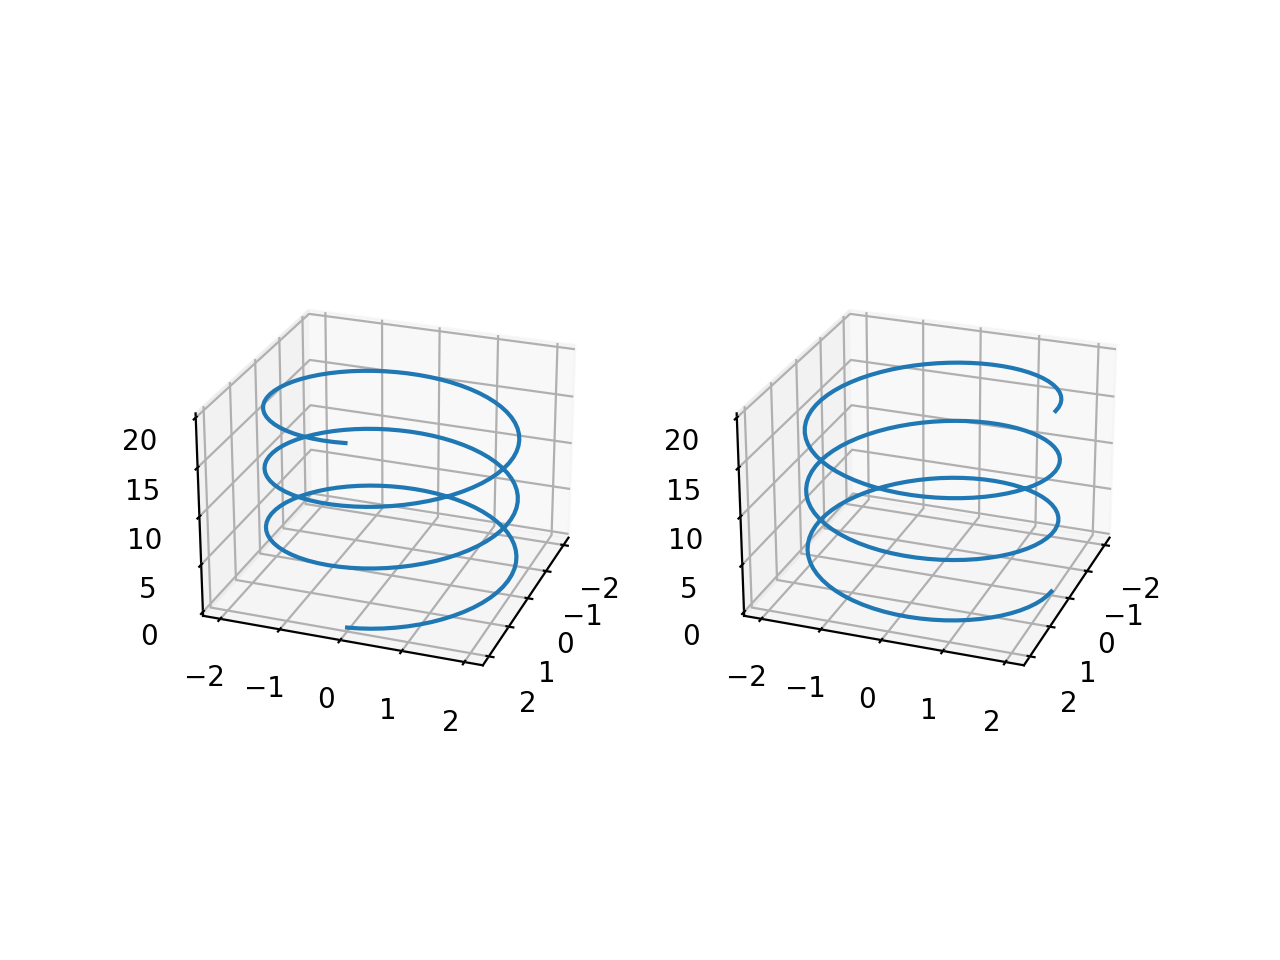
\includegraphics[width=10cm]{figs/duas_helices.png}
 \end{center}

 \section{Orientação}
 
 Circunferência no plano orientada no sentido anti-horário:
 \begin{eqnarray*}
  x(t) &=& \cos(t)\\
  y(t) &=& \sin(t)\\
  %z(t) &=& t
 \end{eqnarray*}
 
\begin{eqnarray*}
  x(0) &=& 1\\
  y(0) &=& 0
 \end{eqnarray*}

 \begin{eqnarray*}
  x(\pi/2) &=& 0\\
  y(\pi/2) &=& 1
 \end{eqnarray*}
 
 
 
 Circunferência no plano orientada no sentido horário:
 \begin{eqnarray*}
  x(t) &=& \sin(t)\\
  y(t) &=& \cos(t)\\
  %z(t) &=& t
 \end{eqnarray*}
 
\begin{eqnarray*}
  x(0) &=& 0\\
  y(0) &=& 1
 \end{eqnarray*}

 \begin{eqnarray*}
  x(\pi/2) &=& 1\\
  y(\pi/2) &=& 0
 \end{eqnarray*}
 

 \section{Torçao - 41min}
 \begin{eqnarray*}
  x(t) &=& \cos(t)\\
  y(t) &=& \sin(t)\\
  z(t) &=& \sin(2t)
 \end{eqnarray*}
 
 \begin{eqnarray*}
  \vec{r}(t) &=& \cos(t)\vec{i}+\sin(t)\vec{j}+ \sin(2t)\vec{k}
 \end{eqnarray*}
 

  \begin{eqnarray*}
\tau = \frac{\vec{r}\!~'\times\vec{r}\!~''\cdot \vec{r}\!~'''}{\|\vec{r}\!~'\times\vec{r}\!~''\|^2}
  \end{eqnarray*}

 \begin{eqnarray*}
  \vec{r}\!~'(t) &=& -\sin(t)\vec{i}+\cos(t)\vec{j}+
  2\cos(2t)\vec{k}\\
  \vec{r}\!~''(t) &=& -\cos(t)\vec{i}-\sin(t)\vec{j}-4\sin(2t)\vec{k}\\
  \vec{r}\!~'''(t) &=& \sin(t)\vec{i}-\cos(t)\vec{j}-
  8\cos(2t)\vec{k}
 \end{eqnarray*}

 \begin{eqnarray*}
  \vec{r}\!~'(\pi/2) &=& -\vec{i}-
  2\vec{k}\\
  \vec{r}\!~''(\pi/2) &=& -\vec{j}\\
  \vec{r}\!~'''(\pi/2) &=& \vec{i}+
  8\vec{k}
 \end{eqnarray*}

 
 \begin{eqnarray*}
\vec{r}\!~'(\pi/2)\times \vec{r}\!~''(\pi/2)=\left(-\vec{i}-
  2\vec{k}\right)\times (-\vec{j})=\vec{k}-2\vec{i}=-2\vec{i}+\vec{k}
  \end{eqnarray*}
 Dica: ijkij
 
\begin{eqnarray*}
   \vec{r}\!~'\times\vec{r}\!~''\cdot \vec{r}\!~'''= \left(-2\vec{i}+\vec{k}\right)\cdot \left(\vec{i}+8\vec{k}\right)= -2+8=6
  \end{eqnarray*}
 

 \begin{eqnarray*}
\|\vec{r}\!~' \times \vec{r}\!~''\|=\|-2\vec{i}+\vec{k}\|=\sqrt{2^2+1^2}=\sqrt{5}
 \end{eqnarray*}
 Finalmente
 $$\tau=\frac{6}{5}$$


 \begin{center}
 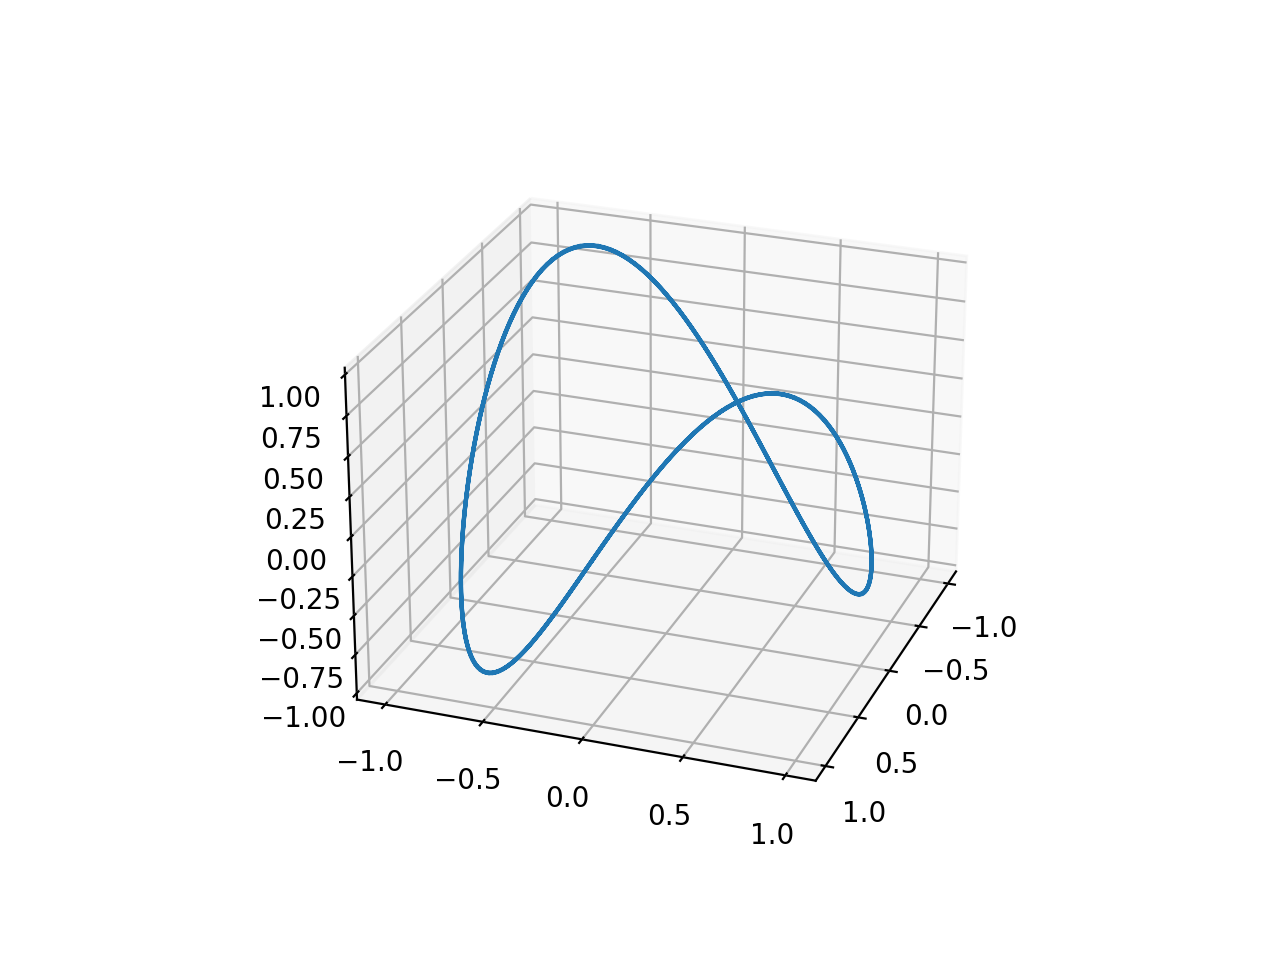
\includegraphics[width=10cm]{figs/curva_cs.png}
 \end{center}
 
 \section{}
\begin{eqnarray*}
  x(t) &=& \int_0^t\cos(\tau^2)d\tau\\
  y(t) &=& \int_0^t\sin(\tau^2)d\tau
\end{eqnarray*}
 
\begin{eqnarray*}
  x'(t) &=& \cos(t^2)\\
  y'(t) &=& \sin(t^2)
\end{eqnarray*}

\begin{eqnarray*}
  x''(t) &=& -2t\sin(t^2)\\
  y''(t) &=& 2t\cos(t^2)
\end{eqnarray*}

Teorema fundamental do cálculo:
$$\frac{d}{dx} \int_a^x f(y)dy = f(x)$$
 
 
 \section{}
 \begin{eqnarray*}
  x(t) &=& \sin(t)\\
  y(t) &=& \cos(t)\\
  z(t) &=& \cos(2t)
 \end{eqnarray*}
 
 Cacule t para $(1,0,-1)$
 
 \begin{eqnarray*}
\sin(t)=1 \Longrightarrow t = \pi/2 + 2k\pi\\
\cos(t)=0 \Longrightarrow t = \pi/2 + k\pi\\
 \cos(2t)=-1 \Longrightarrow 2t = \pi + 2k\pi\\
 \end{eqnarray*}

 \section{Comprimento de arco. 122min}
 
 \begin{eqnarray*}
 \vec{r}(t)&=&2\cos(\pi t)\vec{i}+2\sin(\pi t)\vec{i}-t\vec{k}\\
  \vec{r}\!~'(t)&=&-2\pi\sin(\pi t)\vec{i}+2\pi\cos(\pi t)\vec{i}-\vec{k}\\
  \|\vec{r}\!~'(t)\|&=&\sqrt{(2\pi)^2+1}=\sqrt{4\pi^2+1}
 \end{eqnarray*}
 
 $$L=\int_0^1ds = \int_0^1\|\vec{r}\!~'(t)\|dt=\sqrt{4\pi^2+1}$$
 
%%Dia 28 de agosto
 \section{Curvatura da elipse}.
 
 \begin{center}
 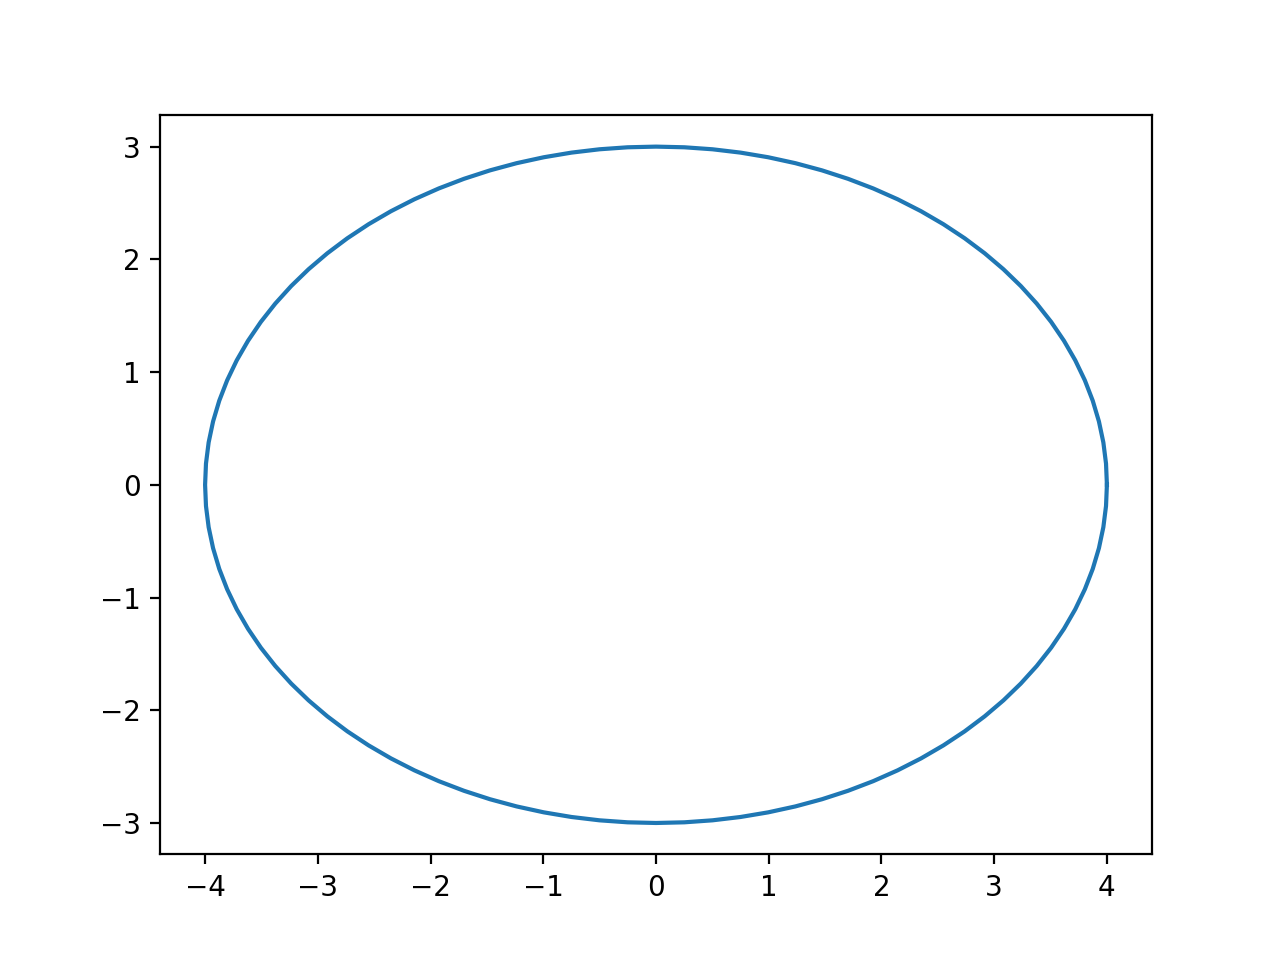
\includegraphics[width=10cm]{figs/elipse.png}
 \end{center}
 
 $$\vec{r}(t)=a\cos(t)\vec{i}+b\sin(t)\vec{j}$$
 onde $a$ e $b$ são constantes positivas. 
 
 \begin{eqnarray*}
  \vec{r}(t)&=&a\cos(t)\vec{i}+b\sin(t)\vec{j}\\
  \vec{r}\!~'(t)&=&-a\sin(t)\vec{i}+b\cos(t)\vec{j}\\
  \vec{r}\!~''(t)&=&-a\cos(t)\vec{i}-b\sin(t)\vec{j}\\
 \end{eqnarray*}

 \begin{eqnarray*}
  \vec{r}\!~'(t)\times \vec{r}\!~''(t)&=&\left(-a\sin(t)\vec{i}+b\cos(t)\vec{j}\right)\times \left(-a\cos(t)\vec{i}-b\sin(t)\vec{j}\right)\\
  &=&ab\sin^2(t)\vec{k}+ab\cos^2(t)\vec{k}= ab\vec{k}
   \end{eqnarray*}

 
 \begin{eqnarray*}
\|\vec{r}\!~'(t)\| &=&\|-a\sin(t)\vec{i}+b\cos^2(t)\vec{j}\|\\
&=& \sqrt{a^2\sin^2(t)+b^2\cos(t)}
 \end{eqnarray*}

E obtemos: 
 \begin{eqnarray*}
  \kappa(t)&=&\frac{\|\vec{r}~\!'(t)\times \vec{r}~\!''(t)\|}{\|\vec{r}~\!'(t)\|^3}\\
  &=&\frac{|ab|}{\left[a^2\sin^2(t)+b^2\cos^2(t)\right]^{3/2}}\\ &=&\frac{ab}{\left[a^2\sin^2(t)+b^2\cos^2(t)\right]^{3/2}}
 \end{eqnarray*}

 Nos vértices $t=0$ e $t=\pi$:
 $$\kappa(0)=\kappa(\pi)=\frac{ab}{(b^2)^{3/2}}=\frac{a}{b^2}$$
 
 
 Nos vértices $t=\pi/2$ e $t=3\pi/2$:
 $$\kappa(\pi/2)=\kappa(3\pi/2)=\frac{ab}{(a^2)^{3/2}}=\frac{b}{a^2}$$
 
 
 \section{Aceleração normal e curvatura}
 Se um pessoa percorre uma trajetória elíptica com semi-eixos $a=100$ e $b=200$ com velocidade escalar constante de 2 m/s. Qual é a aceleração normal máxima.
 $$a_N = \kappa v^2=\kappa_{max} 2^2=4\frac{200}{100^2}=\frac{8}{100}=0,08$$
 
 \section{Campos 53}
 \begin{itemize}
  \item Campos vetoriais e escalares
  \item Campo (vetorial) conservativo. $\vec{F}=\vec{\nabla}\varphi$, $\varphi$ é o potencial. $\vec{\nabla}\times\vec{F}=\vec{0}$.
  \item O campo elétrico é conservativo quando o campo magnético é constante no tempo.
  \end{itemize}

\section{Gradiente (pág 5/5)}
O gradiente de um campo escalar é um campo vetorial. Em cada ponto, é o vetor que aponta na direção e sentido de maior variação e cujo módulo é a máxima derivada direcional:
  $$\frac{\partial f}{\partial \vec{u}}=\vec{u}\cdot\vec{\nabla} f,~~\|\vec{u}\|=1$$ 

  Obs: Direção de máxima derivada direcional é dada pelo vetor unitário (versor):
  $$\vec{u}=\hat{u}=\frac{\vec{\nabla} f}{\|\vec{\nabla} f\|}$$
 
 Direção de mínima derivada direcional (maior valor absoluto e sinal negativo) é dada pelo vetor unitário (versor):
  $$\vec{u}=\hat{u}=-\frac{\vec{\nabla} f}{\|\vec{\nabla} f\|}$$
 
 Se $\vec{u}\cdot \vec{\nabla}f = 0$

 \section{Divergente}
 O divergente de um campo vetorial é o campo escalar dado por:
 $$\vec{\nabla}\cdot \vec{F} = \frac{\partial F_1}{\partial x}+\frac{\partial F_2}{\partial y}+\frac{\partial F_3}{\partial z}$$
 Ex.
 $$     \vec{F}=xy\vec{i}+y^3\vec{j}+xyz^2\vec{k}$$
  \begin{eqnarray*}
 \vec{\nabla}\cdot\vec{F}&=&\frac{\partial }{\partial x}(xy)+\frac{\partial }{\partial y}(y^3)+\frac{\partial }{\partial z}(xyz^2)\\
 &=&y+ 3y^2+2xyz
 \end{eqnarray*}
 
 
 
 \section{}
 
 \begin{eqnarray*}
\vec{r}(t)&=&\int_0^t\cos(\tau^2)d\tau\vec{i}+\int_0^t\sin(\tau^2)d\tau\vec{j}  
 \end{eqnarray*}

 \begin{eqnarray*}
\vec{r}\!~'(t)&=&\cos(t^2)\vec{i}+\sin(t^2)\vec{j}  
 \end{eqnarray*}

 Teorema fundamental do cálculo:
 $$\frac{d}{dt}\int_a^t f(x)dx = f(t)$$
$$\int\cos(t^2)dt \neq \sin(t^2)+C$$
 
 
 \end{document}

